\documentclass[11pt,a4paper]{article}

\usepackage[english,brazilian]{babel}
\usepackage{fontspec}
\defaultfontfeatures{Ligatures=TeX,Scale=MatchLowercase}
\usepackage[a4paper,top=2.25cm,bottom=2.25cm,left=2.45cm,right=2.45cm,headheight=15pt]{geometry}
\usepackage{microtype}
\usepackage{setspace}
\setstretch{1.045}
\setlength{\parindent}{1.1cm}
\setlength{\parskip}{0pt}
\setlength{\emergencystretch}{3em}

\usepackage{amsmath,amssymb}
\usepackage{booktabs,longtable,array,tabularx,makecell}
\usepackage{caption}
\captionsetup{font=small,labelfont=bf,justification=justified,singlelinecheck=false}
\captionsetup[table]{position=top,skip=5pt}
\captionsetup[figure]{position=bottom,skip=6pt}
\usepackage{graphicx}
\usepackage{float,placeins,needspace}
\usepackage{enumitem}
\setlist{itemsep=2pt,topsep=4pt}
\usepackage{xcolor}
\definecolor{ruleblue}{HTML}{416A8A}
\definecolor{softblue}{HTML}{EFF5FA}
\definecolor{softred}{HTML}{FCEFEF}
\usepackage[most]{tcolorbox}
\usepackage{xurl}
\usepackage{fancyhdr}
\pagestyle{fancy}
\fancyhf{}
\fancyhead[L]{\small Suplemento técnico da validação}
\fancyhead[R]{\small Queiroz}
\fancyfoot[C]{\thepage}
\renewcommand{\headrulewidth}{0.3pt}

\usepackage[unicode=true,pdfencoding=auto,psdextra]{hyperref}
\hypersetup{
  colorlinks=true,
  linkcolor=ruleblue,
  urlcolor=ruleblue,
  citecolor=ruleblue,
  pdftitle={Suplemento técnico: validação de grafos de comportamento assistida por agentes de LLM},
  pdfauthor={João Carlos Queiroz},
  pdfsubject={Detalhamento das Campanhas 1--3, GraphForge, modelos, custos, emendas e rastreabilidade},
  pdfkeywords={sistemas tutores inteligentes; grafos de comportamento; CTAT; LLM; GraphForge; suplemento técnico}
}
\usepackage{bookmark}

\newcolumntype{Y}{>{\raggedright\arraybackslash}X}
\newcolumntype{P}[1]{>{\raggedright\arraybackslash}p{#1}}
\newcolumntype{C}[1]{>{\centering\arraybackslash}p{#1}}
\newcolumntype{R}[1]{>{\raggedleft\arraybackslash}p{#1}}
\newcommand{\Rbug}{\ensuremath{R_{\mathrm{bug}}}}
\newcommand{\Rok}{\ensuremath{R_{\mathrm{ok}}}}
\newcommand{\Rbuganchor}{\ensuremath{R_{\mathrm{bug,anchor}}}}
\newcommand{\Rokcompleted}{\ensuremath{r_{\mathrm{ok,completed}}}}
\newcommand{\NA}{\textemdash}
\renewcommand{\thetable}{S\arabic{table}}
\renewcommand{\thefigure}{S\arabic{figure}}
\setcounter{secnumdepth}{2}

\title{\bfseries Suplemento técnico da validação em camadas de grafos de comportamento assistida por agentes de LLM}
\author{João Carlos Queiroz\\\small EducaOFF\\\small \href{mailto:contato@educaoff.com.br}{contato@educaoff.com.br}}
\date{}

\begin{document}
\selectlanguage{brazilian}
\maketitle

\begin{abstract}
Este suplemento preserva o detalhamento técnico que sustenta, mas não deve interromper, a narrativa do artigo principal. São documentados os resultados históricos das Campanhas 1--3, a construção das matrizes de concordância, a bateria comportamental, as sensibilidades, os incidentes que invalidaram análises específicas, os ensaios de engenharia do GraphForge, o registro de modelos e custos e a trilha de emendas da Campanha 4. A antiga matriz agregada da Campanha 1 é corrigida: ela é uma matriz \emph{pooled} de 72 pares exercício--réplica, com 437 ocorrências não independentes, e não uma matriz calculada depois de agregar as três réplicas por exercício. O gabarito correto foi compartilhado pelos dois classificadores, de modo que a célula correto--correto não constitui evidência sobre a geração do caminho correto. A célula surpresa--surpresa é estruturalmente não observável porque a bateria é a união dos catálogos. O suplemento mantém a distinção entre concordância por valor, reconhecimento no estado, integridade estrutural, determinismo e validade pedagógica. Nenhum resultado histórico é combinado estatisticamente com a Campanha 4.

\smallskip\noindent\textbf{Palavras-chave:} grafos de comportamento; CTAT; example tracing; concordância; misconceptions; GraphForge; reprodutibilidade.
\end{abstract}

\section{Função, escopo e relação com o artigo principal}

O artigo principal apresenta a pergunta científica, a Campanha 4 como estudo principal e a síntese sobre a qualidade dos artefatos produzidos pelo fluxo legado da EducaOFF. Este suplemento reúne a trilha técnica necessária para auditar a evolução do instrumento. Ele não introduz uma quinta campanha, não substitui os estimandos principais e não transforma as Campanhas 1--3 em réplicas da Campanha 4.

As quatro campanhas diferem em entrada, runtime, retenção de saídas, modelo estatístico e unidade operacional. Nas Campanhas 1 e 2, o envelope entregue à bancada derivava do mesmo arquivo BRD usado como referência, embora guardas impedissem a passagem de campos comportamentais explícitos. A Campanha 3 construiu a entrada sem ler o conteúdo comportamental do grafo de referência e acrescentou uma bateria independente em parte, mas continuou avaliando o subsistema integrado em uma bancada adaptada. A Campanha 4 preservou as saídas brutas dos agentes implantados, separou agente, extrator e montador e fechou os resultados antes de abrir os BRDs.

Por essa razão, os números históricos têm três funções legítimas: documentar o desenvolvimento do instrumento; mostrar por que cobertura por valor, conformidade no estado e integridade estrutural não são intercambiáveis; e preservar resultados adversos e incidentes que motivaram o protocolo posterior. Eles não autorizam cálculo de tendência temporal, ganho de versão ou média conjunta.

\begin{tcolorbox}[colback=softblue,colframe=ruleblue,title={Regra de leitura}]
Uma métrica histórica responde somente à pergunta e ao artefato para os quais foi construída. Concordância com um catálogo CTAT não é verdade pedagógica universal; ausência de violação estrutural não prova conteúdo correto; determinismo não recupera informação perdida; e nota de LLM-juiz não substitui avaliadores humanos.
\end{tcolorbox}

\section{Fontes, unidades e convenções de reconstrução}

O corpus contém 24 exercícios de frações na reta numérica. Cada exercício possui um arquivo BRD CTAT, metadados e envelopes materializados. Nas Campanhas 1 e 2, cada condição foi executada em três réplicas. Para estimativas macro e intervalos, as réplicas foram agregadas dentro do exercício antes da média entre os 24 exercícios. A matriz \emph{pooled} da Campanha 1 constitui uma exceção descritiva: ela soma as matrizes de 72 pares exercício--réplica para tornar visíveis os territórios de interseção e divergência.

Os dados brutos da Campanha 1 estão em \path{resultados/campanha-2026-07-02/}; os da Campanha 2, em \path{resultados/campanha-2026-07-08-multimodelo/}; e os da Campanha 3, em \path{resultados/campanha3-2026-07-13/}. As reanálises históricas são geradas por \path{analysis/reanalyze.mjs} e \path{analysis/reanalyze-c3.mjs}, com derivados em \path{analysis/derived/reanalise.json} e \path{analysis/derived/reanalise-c3.json}. O artigo e este suplemento usam ponto como separador interno nos arquivos e vírgula na apresentação em português.

A comparação funcional histórica usa uma bateria por par formada pela união de: resposta correta externa, valores errados conceituais da referência e valores errados propostos pelo sistema. A deduplicação ocorre por \path{canonAnswer} dentro de cada par. Frações equivalentes e formas decimais canonicamente iguais são tratadas como a mesma âncora. A opção \path{excludeMechanical=true} remove registros mecânicos da referência. O veredito tem prioridade \emph{erro previsto} sobre \emph{correto} e, na ausência de ambos, \emph{surpresa}.

Essa operação é por valor. Ela não verifica estado CTAT, Selection--Action--Input, ordem do caminho ou remediação. Como o mesmo gabarito correto é fornecido aos dois classificadores, as células associadas à categoria \emph{correto} funcionam principalmente como controle de conflito: verificam se algum catálogo de erro tratou a resposta correta como misconception. Não medem se o agente produziu um caminho correto completo.

\section{Campanha 1: piloto do instrumento integrado}

\subsection{Resultados macro e alcance}

A Campanha 1 avaliou 24 exercícios em três réplicas da bancada integrada. A completude conceitual por valor foi 0,376 (IC95\% 0,309--0,442); a completude bruta, incluindo registros mecânicos, foi 0,234 (0,195--0,273); e a completude de passos foi 0,510 (0,497--0,525). A concordância bruta média de classificação foi 0,396 (0,345--0,449), enquanto o kappa médio foi 0,007 ($-0,069$ a 0,089). A unidade dessas estimativas é o exercício, depois de agregar as réplicas.

\begin{table}[H]
\centering
\caption{Síntese auditada da Campanha 1. As primeiras cinco linhas são médias macro por exercício; a última é uma proporção sobre 66 itens únicos decididos, com intervalo reamostrado por exercício.}
\label{tab:s-c1-summary}
\small
\begin{tabularx}{\textwidth}{@{}Y C{2.7cm}P{5.4cm}@{}}
\toprule
Métrica & Estimativa [IC95\%] & Limite interpretativo \\
\midrule
Completude conceitual por valor & 0,376 [0,309; 0,442] & cobertura do catálogo de um autor, não correção universal \\
Completude bruta & 0,234 [0,195; 0,273] & inclui sentinelas e ações mecânicas \\
Completude de passos & 0,510 [0,497; 0,525] & sensível à granularidade dos grafos \\
Concordância bruta média & 0,396 [0,345; 0,449] & média por exercício; bateria sem verdadeiros negativos \\
Kappa médio de Cohen & 0,007 [$-0,069$; 0,089] & não demonstra concordância além do acaso \\
Excedentes plausíveis segundo GLM-4.5 & 0,833 [0,738; 0,914] & juiz único, decisão por maioria, sem calibração humana \\
\bottomrule
\end{tabularx}
\end{table}

O painel histórico GLM-4.5 classificou como plausíveis 55 dos 66 itens únicos decididos do grupo de excedentes; dois empates foram excluídos. A taxa descreve apenas a decisão daquele juiz sob aquela rubrica. O modelo aprovou 82 de 83 itens da referência e rejeitou os controles de resposta correta e de valor absurdo. O desenho não fornece uma banda humano--humano nem converte plausibilidade textual em validade pedagógica.

\subsection{Matriz \emph{pooled} corrigida}

A Tabela~\ref{tab:s-c1-matrix} soma as baterias de 24 exercícios em três réplicas. Portanto, suas 437 ocorrências não são observações independentes e a referência conceitual de 83 itens é repetida uma vez em cada réplica. A reconstrução por réplica produziu: interseções 32, 29 e 30; itens somente na referência 51, 54 e 53; e itens somente no sistema 40, 38 e 38. As somas são, respectivamente, 91, 158 e 116.

\begin{table}[H]
\centering
\caption{Matriz \emph{pooled} de vereditos por valor na Campanha 1, sobre 72 pares exercício--réplica; linhas: referência CTAT, colunas: sistema.}
\label{tab:s-c1-matrix}
\small
\setlength{\tabcolsep}{6pt}
\begin{tabular}{@{}lrrrr@{}}
\toprule
 & correto & erro previsto & surpresa & total \\
\midrule
correto & 72 & 0 & 0 & 72 \\
erro previsto & 0 & 91 & 158 & 249 \\
surpresa & 0 & 116 & \NA\textsuperscript{a} & 116 \\
\midrule
total & 72 & 207 & 158 & 437 \\
\bottomrule
\end{tabular}
\begin{minipage}{0.96\textwidth}
\footnotesize\emph{Nota.} Contagens \emph{pooled}, não unidades inferenciais independentes. A bateria de cada par é a união da resposta correta externa com os \path{wrongAnswers} dos dois lados, deduplicada por \path{canonAnswer}; registros mecânicos são excluídos (\path{excludeMechanical=true}). O mesmo gabarito correto é fornecido aos dois classificadores. Assim, 72 em correto--correto não demonstra geração do caminho correto; mostra que o catálogo de erros do sistema não entrou em conflito com essas 72 âncoras. \textsuperscript{a}Surpresa--surpresa é não observável por construção: um valor ausente dos dois catálogos não entra na bateria união.
\end{minipage}
\end{table}

Entre as 249 ocorrências de erro conceitual da referência, 91 (36,5\%) também apareceram no sistema e 158 (63,5\%) não foram recuperadas. Entre as 207 ocorrências de erro previstas pelo sistema, 116 (56,0\%) não constavam da referência. Essas 116 não são automaticamente falsas: a referência pode ser incompleta e os excedentes não foram adjudicados por especialistas independentes.

A concordância bruta da matriz \emph{pooled} é $163/437=0,373$ e seu kappa é $-0,033$. Esses valores não são os estimandos macro da Tabela~\ref{tab:s-c1-summary}. A concordância 0,396 e o kappa 0,007 são médias depois da agregação por exercício; a matriz tem função descritiva e de auditoria do mecanismo que deprime o kappa. A ausência de verdadeiros negativos eleva a concordância esperada por acaso, mas não transforma o kappa próximo de zero em resultado favorável.

\begin{figure}[tbp]
  \centering
  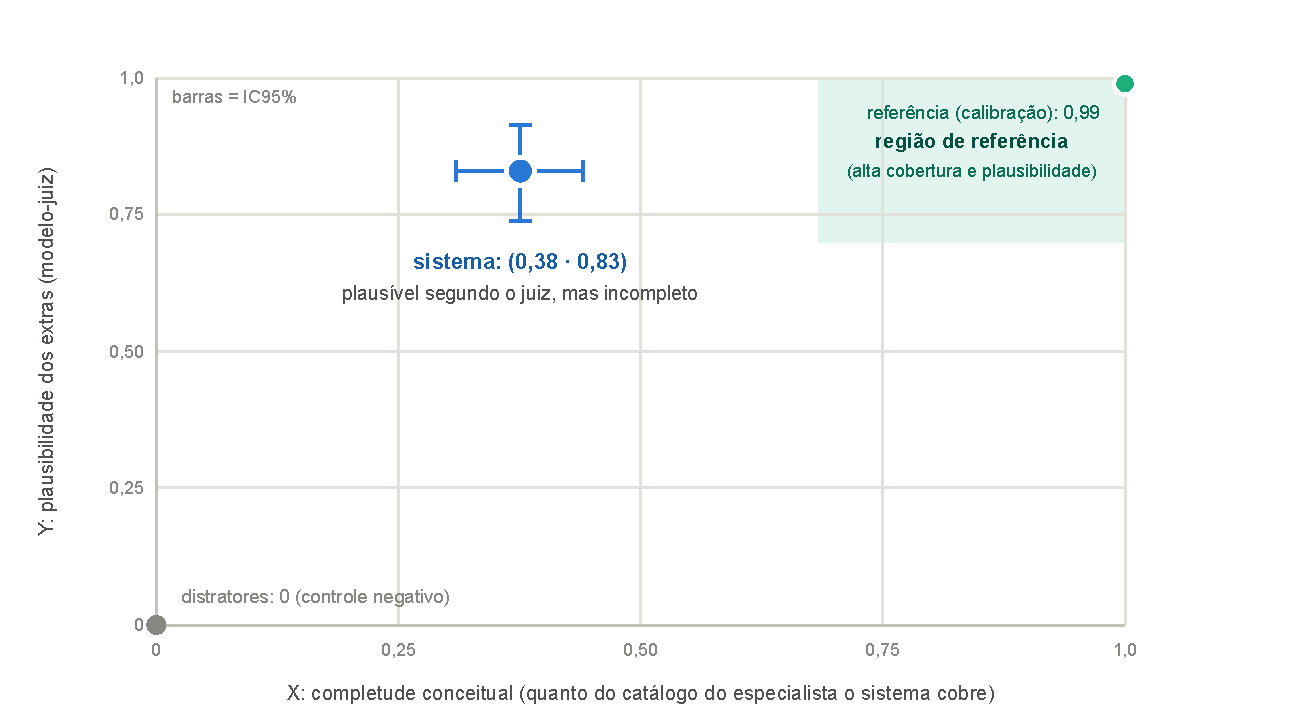
\includegraphics[width=0.84\linewidth]{../v6.0/figures/figura-10.pdf}
  \caption{Síntese histórica da Campanha 1 no plano cobertura--plausibilidade. A ordenada provém de um juiz único e não é probabilidade de validade pedagógica. A figura documenta o instrumento v1 e não representa os desfechos da Campanha 4.}
  \label{fig:s-c1-historical}
\end{figure}
\FloatBarrier

\section{Campanha 2: repetibilidade interna e variação do gerador}

\subsection{Resultados por modelo}

A Campanha 2 repetiu o baseline e substituiu o modelo gerador nos três agentes da bancada. Os braços foram Gemini 3.5 Flash, GLM-5.2, DeepSeek V4 Pro e Claude Sonnet 5. O Gemini repetido obteve completude conceitual 0,368 (0,300--0,442), próxima da Campanha 1, 0,376 (0,309--0,442). Isso é repetibilidade interna no mesmo corpus, não replicação independente.

\begingroup
\footnotesize
\setlength{\tabcolsep}{3pt}
\begin{longtable}{@{}P{3.4cm}C{2.35cm}C{2.35cm}C{2.35cm}C{2.35cm}@{}}
\caption{Resultados históricos por modelo gerador na Campanha 2.}\label{tab:s-c2-models}\\
\toprule
Métrica & Gemini & GLM-5.2 & DeepSeek V4 Pro & Claude Sonnet 5 \\
\midrule
\endfirsthead
\toprule
Métrica & Gemini & GLM-5.2 & DeepSeek V4 Pro & Claude Sonnet 5 \\
\midrule
\endhead
Completude conceitual & 0,368 [0,300; 0,442] & 0,415 [0,323; 0,504] & 0,371 [0,292; 0,454] & 0,416 [0,339; 0,488] \\
Completude de passos & 0,508 [0,493; 0,523] & 0,501 [0,479; 0,521] & 0,477 [0,458; 0,496] & 0,500 [0,487; 0,516] \\
Kappa médio & 0,051 & $-0,027$ & $-0,074$ & $-0,033$ \\
Excedentes plausíveis segundo Mistral & 0,742 & 0,777 & 0,730 & 0,733 \\
\bottomrule
\end{longtable}
\endgroup

Nenhuma diferença de completude conceitual contra o baseline sobreviveu ao ajuste de Holm. Isso não demonstra equivalência: os intervalos das diferenças ainda admitem efeitos relevantes. Entre métricas secundárias, somente a menor completude de passos do DeepSeek sobreviveu ao ajuste. Os níveis do juiz Mistral da Campanha 2 não são diretamente comparáveis aos níveis do GLM-4.5 da Campanha 1.

\subsection{Cobertura por tipo e múltiplas chamadas}

A referência continha 83 âncoras conceituais: 30 frações incorretas, 24 numeradores isolados, 24 denominadores isolados e cinco outros inteiros. O denominador isolado foi o ponto cego mais persistente. A união de réplicas elevou cobertura, mas também ampliou o conjunto que exigiria revisão.

\begin{table}[H]
\centering
\caption{Cobertura histórica por tipo de erro no baseline da Campanha 2.}
\label{tab:s-c2-error-types}
\small
\begin{tabularx}{\textwidth}{@{}Y R{1.4cm}R{2.3cm}R{2.3cm}@{}}
\toprule
Tipo na referência & N & Uma execução & União de três \\
\midrule
Fração incorreta, por exemplo $2/4$ quando a resposta é $3/4$ & 30 & 39\% & 73\% \\
Numerador isolado, por exemplo ``3'' & 24 & 50\% & 79\% \\
Denominador isolado, por exemplo ``4'' & 24 & 14\% & 33\% \\
Outros inteiros & 5 & 73\% & 80\% \\
\midrule
\textbf{Total} & \textbf{83} & \textbf{37\%} & \textbf{64\%} \\
\bottomrule
\end{tabularx}
\end{table}

Em um experimento auxiliar separado da Campanha 2, com amostrador e número de chamadas próprios, uma curva até $K=5$ apresentou ganhos decrescentes: 31,3\% em $K=1$, 43,2\% em $K=2$, 48,9\% em $K=3$, 52,6\% em $K=4$ e 55,6\% em $K=5$. Esses valores vêm de \path{resultados/saturation-curve-2026-07-10.json} e não foram recalculados como braço da reanálise C2. Repetir chamadas aumenta diversidade potencial, mas não garante validade dos excedentes, preservação pelo extrator ou baixo custo de revisão.

\subsection{Comparações pareadas selecionadas}

As diferenças foram calculadas dentro do exercício e avaliadas por permutação exata com ajuste de Holm. A ausência de diferença detectada não é um teste de equivalência nem de não inferioridade.

\begingroup
\small
\setlength{\tabcolsep}{3pt}
\begin{longtable}{@{}P{5.2cm}C{3.1cm}C{1.7cm}C{1.7cm}P{2.3cm}@{}}
\caption{Comparações históricas contra o Gemini na Campanha 2.}\label{tab:s-c2-tests}\\
\toprule
Comparação & $\Delta$ médio [IC95\%] & p exato & p-Holm & Resultado \\
\midrule
\endfirsthead
\toprule
Comparação & $\Delta$ médio [IC95\%] & p exato & p-Holm & Resultado \\
\midrule
\endhead
GLM-5.2, completude conceitual & $+0,047$ [$-0,048$; 0,143] & 0,381 & 0,988 & não detectado \\
DeepSeek, completude conceitual & $+0,003$ [$-0,089$; 0,091] & 0,957 & 0,988 & não detectado \\
Claude Sonnet 5, completude conceitual & $+0,047$ [$-0,038$; 0,142] & 0,329 & 0,988 & não detectado \\
DeepSeek, completude de passos & $-0,031$ [$-0,047$; $-0,015$] & 0,003 & 0,035 & diferença detectada \\
DeepSeek, F1 estrutural & $-0,056$ [$-0,092$; $-0,023$] & 0,005 & 0,052 & diferença não detectada após Holm \\
Claude Sonnet 5, inclusão de traços & $+0,059$ [0,017; 0,101] & 0,011 & 0,114 & não após Holm \\
\bottomrule
\end{longtable}
\endgroup

\section{Campanha 3: bateria comportamental e conformidade integrada}

\subsection{Bateria, condições e estimandos}

A Campanha 3 removeu o conteúdo comportamental do BRD da entrada entregue à autoria. Sua bateria de 636 itens, contudo, não era integralmente independente da referência: 240 itens vinham diretamente dela, 135 eram mutações de traços de referência e 261 eram sondas construídas a partir do gabarito. A Campanha 3 avaliou nove condições, três réplicas e 24 exercícios, totalizando 648 autorias.

\begin{table}[H]
\centering
\caption{Composição da bateria comportamental da Campanha 3.}
\label{tab:s-c3-battery}
\small
\begin{tabularx}{\textwidth}{@{}P{3.4cm}Y R{1.8cm}@{}}
\toprule
Família & Origem e função & Itens \\
\midrule
A -- referência & 24 traços corretos, 192 ações buggy e 24 pedidos de dica & 240 \\
B -- mutações & traços perturbados derivados da referência & 135 \\
C -- sondas & itens de domínio oriundos do gabarito; verdadeiros negativos & 261 \\
\midrule
Total & 24 a 28 itens por exercício & 636 \\
\bottomrule
\end{tabularx}
\end{table}

Para uma ação buggy, \Rbug{} verifica se o executor a aceita como erro previsto no estado correspondente. Para um caminho correto, \Rok{} exige aceitação passo a passo e chegada ao objetivo. A sensibilidade \Rbuganchor{} exclui 42 ações mecânicas que não puderam ser ancoradas, deixando 150 ações; \Rokcompleted{} relaxa a igualdade do caminho e exige somente conclusão. A cobertura por valor ignora estado e ordem, sendo secundária.

As condições foram: baseline Gemini; geração com GLM-5.2; geração com DeepSeek V4 Pro; catálogo interno; limite de seis candidatos; saturação textual; entrada DOM; entrada por screenshot; e chamada única. Os dois braços multimodais tinham falhas de pareamento e permanecem somente para trilha de auditoria.

\subsection{Resultados nas nove condições}

\begingroup
\footnotesize
\setlength{\tabcolsep}{3pt}
\begin{longtable}{@{}P{4.2cm}C{2.5cm}C{1.4cm}C{2.6cm}C{2.5cm}@{}}
\caption{Desfechos e cobertura nas nove condições da Campanha 3.}\label{tab:s-c3-arms}\\
\toprule
Condição & \Rbug{} [IC95\%] & \Rok{} & Cobertura [IC95\%] & Sinal mole \\
\midrule
\endfirsthead
\toprule
Condição & \Rbug{} [IC95\%] & \Rok{} & Cobertura [IC95\%] & Sinal mole \\
\midrule
\endhead
Baseline Gemini & 0,054 [0,016; 0,095] & 0 & 0,243 [0,163; 0,324] & 0/72 \\
GLM-5.2 & 0,040 [0,016; 0,068] & 0 & 0,178 [0,122; 0,236] & 0/72 \\
DeepSeek V4 Pro & 0,023 [0,010; 0,036] & 0 & 0,199 [0,143; 0,260] & 0/72 \\
Catálogo interno & 0,021 [0,005; 0,040] & 0 & 0,215 [0,152; 0,282] & 0/72 \\
Limite de seis candidatos & 0,078 [0,028; 0,134] & 0 & 0,419 [0,342; 0,495] & 61/72 \\
Saturação textual & 0,042 [0,010; 0,082] & 0 & 0,238 [0,171; 0,307] & 0/72 \\
DOM inválido para inferência & 0,028 [0,005; 0,056] & 0 & 0,207 [0,134; 0,279] & 0/72 \\
Screenshot inválido para inferência & 0,023 [0,009; 0,036] & 0 & 0,251 [0,180; 0,324] & 0/72 \\
Chamada única & 0,010 [0; 0,024] & 0 & 0,203 [0,147; 0,264] & 1/72 \\
\bottomrule
\end{longtable}
\endgroup

No baseline, \Rbug{} foi 0,054 (0,016--0,095), \Rok{} foi zero e a cobertura por valor foi 0,243 (0,163--0,324). O limite de seis candidatos elevou a cobertura em 17,7 pontos contra o baseline (p-Holm $=2,4\times10^{-5}$), mas não demonstrou ganho em reconhecimento no estado e coincidiu com 61 de 72 sinais moles. Em todas as 648 autorias, não houve violação dura; 62 (9,6\%) acionaram sinal mole, quase todos na condição de seis candidatos.

Quantidade, portanto, alterou um estimando de catálogo sem melhorar de forma demonstrável o estimando comportamental. Esse contraste antecipa o resultado da Campanha 4: gerar conteúdo não garante que ele esteja corretamente localizado, transportado ou utilizável pelo tutor.

\subsection{Sensibilidades e reconstrução}

\begingroup
\footnotesize
\setlength{\tabcolsep}{3pt}
\begin{longtable}{@{}P{5.0cm}C{3.7cm}C{3.7cm}@{}}
\caption{Sensibilidades exploratórias da Campanha 3.}\label{tab:s-c3-sens}\\
\toprule
Condição & \Rbuganchor{} [IC95\%] & \Rokcompleted{} [IC95\%] \\
\midrule
\endfirsthead
\toprule
Condição & \Rbuganchor{} [IC95\%] & \Rokcompleted{} [IC95\%] \\
\midrule
\endhead
Baseline & 0,065 [0,020; 0,113] & 0,069 [0; 0,167] \\
GLM-5.2 & 0,048 [0,019; 0,080] & 0,042 [0; 0,111] \\
DeepSeek & 0,027 [0,013; 0,044] & 0,097 [0,042; 0,167] \\
Catálogo interno & 0,025 [0,006; 0,049] & 0,097 [0; 0,222] \\
Limite de seis candidatos & 0,094 [0,037; 0,157] & 0,125 [0,042; 0,236] \\
Saturação & 0,050 [0,014; 0,096] & 0,083 [0; 0,194] \\
DOM, não interpretável & 0,033 [0,007; 0,066] & 0,292 [0,125; 0,472] \\
Screenshot, não interpretável & 0,030 [0,012; 0,049] & 0,014 [0; 0,042] \\
Chamada única & 0,014 [0; 0,032] & 0 [0; 0] \\
\bottomrule
\end{longtable}
\endgroup

Os relatórios históricos não retiveram o veredito de cada ação. O numerador de \Rbug{} foi reconstruído a partir da taxa ancorável, do denominador conhecido e do arredondamento armazenado. O script testa se existe um único inteiro compatível com a taxa publicada dentro da tolerância. Essa reconstrução é auditável, mas é inferior à retenção item a item; por isso, a Campanha 3 permanece evidência histórica secundária.

Os intervalos usam o exercício como cluster, depois da média das réplicas. Eles descrevem este corpus e este mecanismo de reamostragem. Não definem uma população de STIs, autores ou domínios. Os braços DOM e screenshot não recebem interpretação causal, ainda que seus valores permaneçam nas tabelas para evitar apagamento retrospectivo.

\section{Análises invalidadas e incidentes preservados}

\begin{enumerate}
  \item \textbf{Envelope v1 derivado do BRD.} A entrada das Campanhas 1--2 e a referência provinham do mesmo arquivo. Guardas removiam campos proibidos, mas não demonstravam independência semântica completa.
  \item \textbf{Braço DOM da Campanha 3.} A representação compartilhada continha um enunciado veterinário alheio ao corpus. O contraste não mede efeito de DOM corretamente pareado.
  \item \textbf{Braço screenshot da Campanha 3.} A imagem de \path{00bubble} foi reutilizada nos 24 exercícios. O contraste não mede efeito visual específico de cada problema.
  \item \textbf{Painel da Campanha 3.} O coletor esperava \path{extras}, enquanto os relatórios armazenavam \path{extra}. Os 179 itens julgados continham 83 itens da referência e 96 controles, mas nenhum excedente do sistema. Seus kappas não apoiam alegações sobre os agentes.
  \item \textbf{Denominador de \Rbug{}.} A primeira implementação excluiu 42 ações mecânicas. A análise corrigida restaura as 192 ações planejadas no desfecho principal e preserva as 150 ancoráveis como sensibilidade.
  \item \textbf{Lançamentos técnicos do painel C4.} As versões v1, v2 e v4 foram excluídas integralmente por incompatibilidades de schema, gramática e composição. Nenhum escore foi reaproveitado no painel v5.
  \item \textbf{Concordância degenerada do painel C4.} Dez dimensões constantes eram mostradas como alfa ou kappa igual a 1. A errata v5.1 marca esses coeficientes como não estimáveis; as notas brutas não mudaram.
\end{enumerate}

Preservar um incidente não o torna evidência válida. Sua função é documentar a cadeia de decisões, impedir seleção retrospectiva favorável e mostrar quais fragilidades foram corrigidas em campanhas posteriores. As análises invalidadas não entram na conclusão consolidada do artigo principal.

\section{Engenharia, verificação e limites do GraphForge}

O GraphForge recebe uma configuração já reduzida pelo extrator e cria nós, arestas, scaffolds e manifestos. O verificador estrutural procura violações duras, como ciclo fora de remediação, nó inalcançável, beco sem saída, scaffold ou aresta órfãos e ausência de início ou objetivo. Sinais moles, como ramificação excessiva, indicam complexidade e necessidade de revisão, não necessariamente invalidade.

\begin{figure}[tbp]
  \centering
  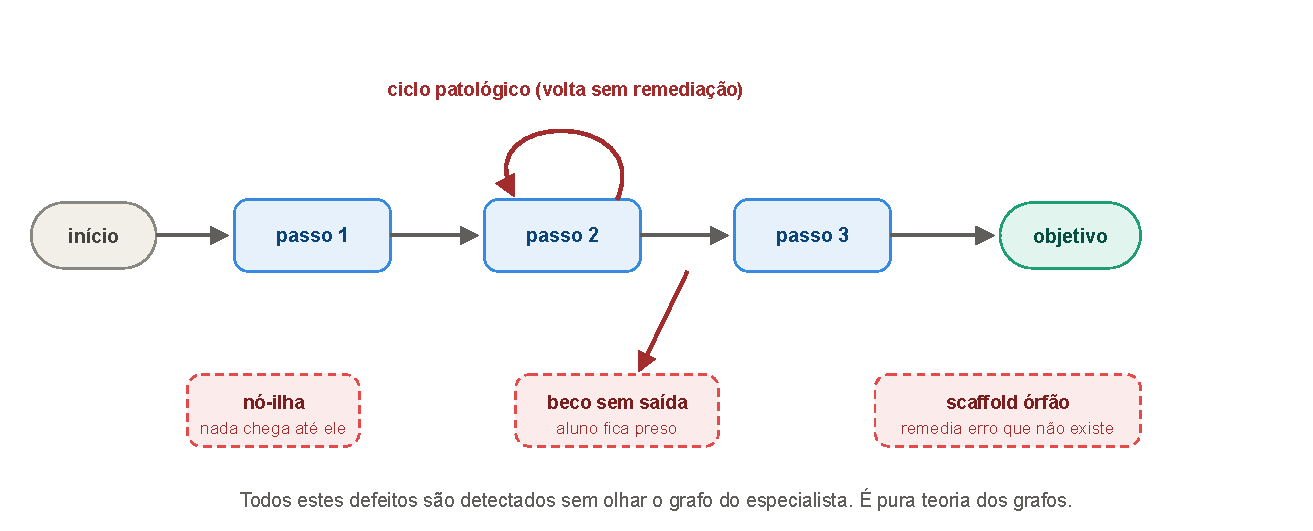
\includegraphics[width=0.89\linewidth]{../v6.0/figures/figura-08.pdf}
  \caption{Exemplos conceituais de violações estruturais procuradas pelo verificador. A ausência desses defeitos não implica conteúdo semanticamente ou pedagogicamente correto.}
  \label{fig:s-structural-defects}
\end{figure}
\FloatBarrier

\begingroup
\small
\setlength{\tabcolsep}{3pt}
\begin{longtable}{@{}P{3.4cm}P{6.0cm}P{4.8cm}@{}}
\caption{Camadas de evidência estrutural do GraphForge.}\label{tab:s-graphforge}\\
\toprule
Ensaio & Resultado & Alegação permitida \\
\midrule
\endfirsthead
\toprule
Ensaio & Resultado & Alegação permitida \\
\midrule
\endhead
Testes de propriedades & 10.000 configurações aleatórias sem violação dura implementada & robustez observada dentro da taxonomia e do gerador de casos \\
Mutation testing & 260/260 mutantes detectados em dez classes; bases intactas sem sinal espúrio & sensibilidade e especificidade para as mutações cobertas \\
Campanha 3 & 0/648 violações duras; 62/648 sinais moles & conformidade estrutural dura nos grafos observados; alertas de complexidade persistem \\
Campanha 4 & 34/34 pares de reexecução idênticos & determinismo observado nas configurações operacional e de capacidade \\
Transporte C4 & perdas antes e depois da configuração & o montador não recupera campos que não recebe \\
\bottomrule
\end{longtable}
\endgroup

Os testes de propriedades cobrem a implementação e a distribuição de configurações gerada pelo teste; não provam ausência de defeitos desconhecidos. O mutation testing mostra que o verificador detecta as dez classes injetadas, não todos os defeitos possíveis. A Campanha 3 mostra conformidade observada com invariantes duras, mas a condição de seis candidatos produziu quase todos os alertas de complexidade. A Campanha 4 demonstra identidade byte a byte em reexecuções, não correção do conteúdo.

A fronteira de responsabilidade é essencial. O GraphForge pode montar exatamente uma topologia alimentada por conteúdo incompleto, e não tem como reconstruir \path{problemId}, localização diagnóstica, nível de dica ou item truncado antes de sua chamada. Integridade estrutural, schema, concordância com referência, retenção de campos, segurança das dicas e revisão pedagógica devem permanecer gates separados.

\section{Registro de modelos, funções e custos}

\begingroup
\footnotesize
\setlength{\tabcolsep}{3pt}
\begin{longtable}{@{}P{1.25cm}P{3.0cm}P{4.1cm}P{3.7cm}P{2.2cm}@{}}
\caption{Modelos e custos por campanha; valores históricos aproximados não devem ser somados como cobrança exata.}\label{tab:s-model-costs}\\
\toprule
Fase & Objeto & Gerador(es) & Juiz(es) & Custo declarado \\
\midrule
\endfirsthead
\toprule
Fase & Objeto & Gerador(es) & Juiz(es) & Custo declarado \\
\midrule
\endhead
C1 & bancada integrada & Gemini 3.5 Flash & GLM-4.5 & aprox. US\$ 4 \\
C2 & robustez histórica & Gemini 3.5 Flash; GLM-5.2; DeepSeek V4 Pro; Claude Sonnet 5 & Mistral Large comum aos braços & aprox. US\$ 30 \\
C3 & conformidade, ablações, ensemble, painel e smoke tests & Gemini; braços GLM e DeepSeek; ablações & Mistral Large 2512; Qwen 3.7 Plus; Llama 4 Maverick, sobre referência e controles & US\$ 16,72 em 1.970 chamadas \\
C4 geração & agentes implantados & Gemini 3.5 Flash & não aplicável & US\$ 1,9540 \\
C4 painel final & saídas congeladas & não aplicável & GLM-5.2; Qwen 3.7 Plus; DeepSeek V4 Pro & US\$ 1,2432 conservador \\
C4 excluídos & testes técnicos & não aplicável & composições anteriores & US\$ 2,2211 conhecido, incompleto \\
\bottomrule
\end{longtable}
\endgroup

Os custos aproximados de C1 e C2 vêm da narrativa operacional e não possuem journal suficiente para reconciliação independente. A Campanha 3 reconcilia 1.970 registros: 1.325 chamadas das nove condições, 240 do ensemble, 393 do painel e 12 de \emph{smoke test}. Ela contém dois erros primários seguidos de fallback bem-sucedido; houve zero falha final de autoria, não zero falha de chamada. O painel C3 recebeu referências e controles, não excedentes do sistema. Os valores de C4 separam geração, painel final e lançamentos excluídos.

Claude e GPT não participaram do painel final da Campanha 4. Claude aparece como gerador histórico da Campanha 2 e em lançamento técnico excluído; GPT aparece apenas em planejamento e lançamento excluído. A mudança do painel não altera as saídas Gemini, as métricas determinísticas ou o GraphForge; altera somente a evidência subjetiva auxiliar e, por isso, é declarada como decisão pós-registro.

Identificadores comerciais de modelos não congelam os pesos remotos. Mesmo quando código, prompts e respostas são preservados por hash, o provedor pode atualizar uma rota sob o mesmo nome. A reprodução offline das métricas é mais forte do que a reprodução externa da geração.

\section{Desvios, emendas e decisões pós-registro}

O congelamento da Campanha 4 foi local e baseado em hashes. As métricas e o protocolo inicial do painel foram congelados antes da primeira chamada paga; três estados da réplica 1 foram então executados como piloto e retidos. O plano das chamadas restantes foi formalizado após esse piloto sem inspeção das métricas de qualidade. A campanha é exploratória e auditável, não um pré-registro integral concluído antes de qualquer dado.

\begingroup
\footnotesize
\setlength{\tabcolsep}{3pt}
\begin{longtable}{@{}P{1.9cm}P{2.8cm}P{5.3cm}P{3.8cm}@{}}
\caption{Trilha resumida de emendas da Campanha 4.}\label{tab:s-amendments}\\
\toprule
Momento & Emenda & Motivo & Efeito analítico \\
\midrule
\endfirsthead
\toprule
Momento & Emenda & Motivo & Efeito analítico \\
\midrule
\endhead
Pré-geração & métricas v2 & contrato multi-problema, placeholders e ausência de estado/SAI & estimandos por \path{problemId}; 3b por valor; 3c estrito; transporte por campo \\
Pós-falha & retomada limitada & JSON 3b malformado no grupo 5 & estado falho não repetido; grupo 6 independente autorizado \\
Pós-resultado & errata v2.1 & vetor incorreto em quatro taxas de campo do 3a & apenas taxas descritivas corrigidas; estimandos e contagens inalterados \\
Pós-auditoria & sensibilidade por batch & quatro exercícios compartilham cada chamada & ICs descritivos por seis clusters; não substituem a análise registrada \\
Pós-auditoria & quarto KC & gate inicial enumerava três de quatro KCs & atestação pós-hoc; enriquecimento efetivo vazio; estimandos inalterados \\
Pré-painel final & schemas v2/v3 & incompatibilidade de keywords e gramáticas por unidade & lançamentos parciais excluídos; schemas estáveis por papel \\
Pré-painel final & modelos v4/v5 & retirada de Claude e GPT por custo & painel reiniciado com GLM, Qwen e DeepSeek; composição pós-registro \\
Pós-auditoria & errata v5.1 & categoria única exibida como alfa/kappa 1 & coeficientes degenerados marcados como não estimáveis; escores inalterados \\
\bottomrule
\end{longtable}
\endgroup

Na falha do grupo 5, a resposta 3a havia sido parseada, a resposta 3b era JSON malformado e o 3c não foi chamado. A política atômica manteve a unidade falha como ausência/zero na análise por intenção de executar, sem retry ou reparo. A execução posterior do grupo 6 já estava autorizada como grupo independente e não reabriu o grupo falho.

A errata de métricas v2.1 corrige as taxas por campo \path{step}, \path{action}, \path{result} e \path{kcUsed} do 3a. Contagens de itens, truncamento e desfechos principais não mudaram. A sensibilidade por batch foi acrescentada porque quatro exercícios compartilham uma chamada; com apenas seis clusters, seus intervalos também são instáveis e permanecem descritivos.

O gate inicial cobriu três dos quatro KCs presentes nas fixtures. No snapshot local, a consulta do quarto KC retornou HTTP 404; o cliente converteu a resposta para \path{null} e, em seguida, para vetor vazio. A verificação operacional pós-hoc na implantação retornou HTTP 200 com o mesmo vetor vazio efetivo. Como as respostas HTTP brutas da VPS não foram preservadas, a afirmação é uma atestação operacional, não reprodução externa independente.

\section{Rastreabilidade, hashes e reprodução}

O repositório canônico é \href{https://github.com/Joaoqueiroz-silva/sti-graph-validation}{github.com/Joaoqueiroz-silva/sti-graph-validation}. A análise determinística da Campanha 4 está em \path{resultados/campanha4-2026-07-15/campaign4-final-analysis-v2.1.json}; o painel final está em \path{resultados/campanha4-2026-07-15/judge-panel-v5/}; e a reanálise histórica que gera a matriz corrigida está em \path{analysis/derived/reanalise.json}. O manifesto global da versão vigente é \path{protocol/frozen/MANIFEST-v6.1.sha256}; \path{MANIFEST-v6.0.sha256} permanece imutável como manifesto histórico da v6.0.

Para evitar duas listas concorrentes, a relação integral de hashes deve ser lida nos manifestos versionados do repositório. A Tabela~\ref{tab:s-hashes} repete somente os identificadores necessários para ligar este suplemento à coleta principal.

\begingroup
\footnotesize
\setlength{\tabcolsep}{3pt}
\begin{longtable}{@{}P{4.1cm}p{10.4cm}@{}}
\caption{Hashes SHA-256 centrais por remissão ao artigo principal e aos manifestos.}\label{tab:s-hashes}\\
\toprule
Artefato & SHA-256 \\
\midrule
\endfirsthead
\toprule
Artefato & SHA-256 \\
\midrule
\endhead
Imagem de produção & \path{15b29e8063099d40fc62899da2795db6e97d3e252e486315428a0690bb9abf5b} \\
Plano de execução & \path{77de38a7bfe25f6dcfb34527081e9b5f73de4b1316ebd414f6129677aae3a074} \\
Código de métricas v2.1 & \path{a228f60e8838055c69e90e91e671ca0653339c8c3af5e2b6b582e98eedec9be2} \\
Análise determinística final & \path{dae582fd1179b20b7b42472bcb84bb6075b2fce7d813a61d2e0f6693f0df9b17} \\
Sensibilidade por batch & \path{1ae514350fc2afc53d7e7c65783eea207f713a4f443a32aec6b62c1c5c992fe4} \\
Manifesto de conclusão & \path{3568b8dc690d916a7857896efc753845dde18ef394e7144062e650fc73fc59c0} \\
Manifesto de redação pública & \path{7445c9dd0f3f511be7ef8bd53ca17cd9ce7488fddc6eec719384d13807146aba} \\
Análise corrigida do painel v5.1 & \path{f32583a08d20ececda98d1e7ff0d117b7d6e0402d7db55b082ad373146addd6c} \\
\bottomrule
\end{longtable}
\endgroup

As cópias públicas dos resultados C4 removem apenas metadados de conta do OpenRouter: saldo, uso acumulado, rótulo e sufixo de credencial. Saídas científicas, modelos, tokens, custos por chamada e falhas permanecem. O manifesto de redação liga os hashes privados originais aos hashes públicos sem expor esses metadados.

O depósito permite recalcular offline métricas, tabelas e sensibilidades. A coleta externa integral ainda depende de uma imagem publicada ou de um snapshot fonte reproduzível. O digest local identifica a imagem usada, mas ela não está disponível como arquivo OCI ou em registry público. Hashes de código tampouco congelam pesos de modelos comerciais remotos.

Os BRDs já constam do histórico remoto, mas hash e disponibilidade técnica não demonstram licença de redistribuição. Autoria, instituição, data e licença do corpus precisam ser regularizadas antes de um benchmark aberto. Até lá, uma release arquivística deve excluir o corpus e seu histórico ou permanecer privada.

\section{Síntese dos limites históricos}

As Campanhas 1 e 2 mostram cobertura parcial e diversidade entre chamadas, mas usam entrada derivada do mesmo BRD e uma bateria união sem verdadeiros negativos. A matriz corrigida evidencia que 91 de 249 ocorrências de erro da referência coincidiram por valor com o sistema; ela não avalia o caminho correto, pois o gabarito foi compartilhado. A Campanha 2 mostra que trocar o modelo não removeu de forma demonstrável o teto de cobertura.

A Campanha 3 melhora a independência da entrada e introduz estado, ações buggy e sondas. Seus resultados mostram baixa conformidade comportamental integrada, ainda que os grafos satisfaçam invariantes duras. A condição de seis candidatos aumenta cobertura por valor ao custo de mais alertas de complexidade. Incidentes de DOM, screenshot e painel impedem interpretações específicas, mas sua preservação fortalece a auditabilidade.

Os ensaios do GraphForge sustentam robustez para as invariantes implementadas, detecção das mutações cobertas e determinismo observado. Eles não estabelecem qualidade semântica. Modelos-juízes históricos e o painel da Campanha 4 oferecem apenas triagem auxiliar. Em conjunto, o material suplementar explica por que o artigo principal adota validação em camadas e por que a versão auditada deve ser tratada como apoio à autoria, não como mecanismo autônomo de aprovação pedagógica.

\end{document}
